\section{Read-out and data processing (20p.)}
n this section we give an overview of data processing from the detector read-out to the creation of analysis object data (see Fig. \ref{fig:02dp})
and then
focus on the processing steps that are synchronous with data taking.
The continuous read-out of the large majority of the detectors without rejecting 
events, is one of the most important changes with respect to Runs~1+2. As explained in 
detail in section \ref{physics_motivation}, it allows to 
record the maximum statistics for physics signals for which dedicated triggering is 
not feasible. At the projected peak Pb--Pb interaction rate of 50~kHz the data throughput from the detectors is expected to be {\color{blue} 3.75~TB/s}, approximately a factor of 50 higher than during Run 2.

In order to minimize the costs and compute time of the online and offline systems
for data processing and storage, the ALICE Computing Model for Runs~3+4 is designed 
for a maximum reduction of the data volume synchronous with the data taking. 
This task is achieved in two processing steps on the ALICE online/offline facility (${\rm O}^2$) located at Point~2.
It consists of two types of compute nodes, the First Level Processors (FLP) located in
the experiment access shaft (CR1) and the Event Processing Nodes (EPN) at CR0. In
addition to the compute
nodes it provides networking, data storage as well as interfaces with the Grid and the
permanent data
store at the Tier~0. For more technical details on these clusters, see sections
\ref{sec:flp} and \ref{sec: epn}.

The upgraded online system supports both continuous and triggered read-out. Not
all sub-systems will be capable of reading the full event rate. These detectors will
therefore be read out whenever they are not busy. Triggered read-out will be also used for commissioning and calibration runs. Data produced by the detectors are transferred to the common read-out units (CRU). The triggered data will be tagged with the triggered LHC bunch-crossing while the continuous streams of data samples are tagged by the so called heartbeat frame (HBF) IDs and the IDs of the Time Frames (TF) containing fixed amount of HBFs.
The HBF has a duration of one LHC orbit ($\approx 89.4\; \mu s$) and is synchronized with the LHC clock. A TF corresponds to 128-256 orbits (11--22~ms) and contains at the peak luminosity 550-1100 collisions.
The data are compressed and multiplexed
in the CRUs and transferred to the memory of the FLPs.

The 272 FLPs perform a
first level of data compression to 635~GB/s by zero suppression as well as
calibration
tasks based on local information from the part of the detector they serve, for example base-line
correction. The calibration objects will be stored in the Calibration and Constants Data Base (CCDB)
and from there they will be read by the following processing stages.
HBFs belonging to the same TF are disentangled to sub-time frames (STF) and dispatched to the next
EPN ready to accept the data.
A dedicated FLP collects and processes data from the Detector Control System (DCS). These data will
be used by the detectors to prepare condition objects with information of its interest and will be
stored in the CCDB and used during reconstruction and simulation.


\begin{figure*}[hbtp]
  \begin{center}
    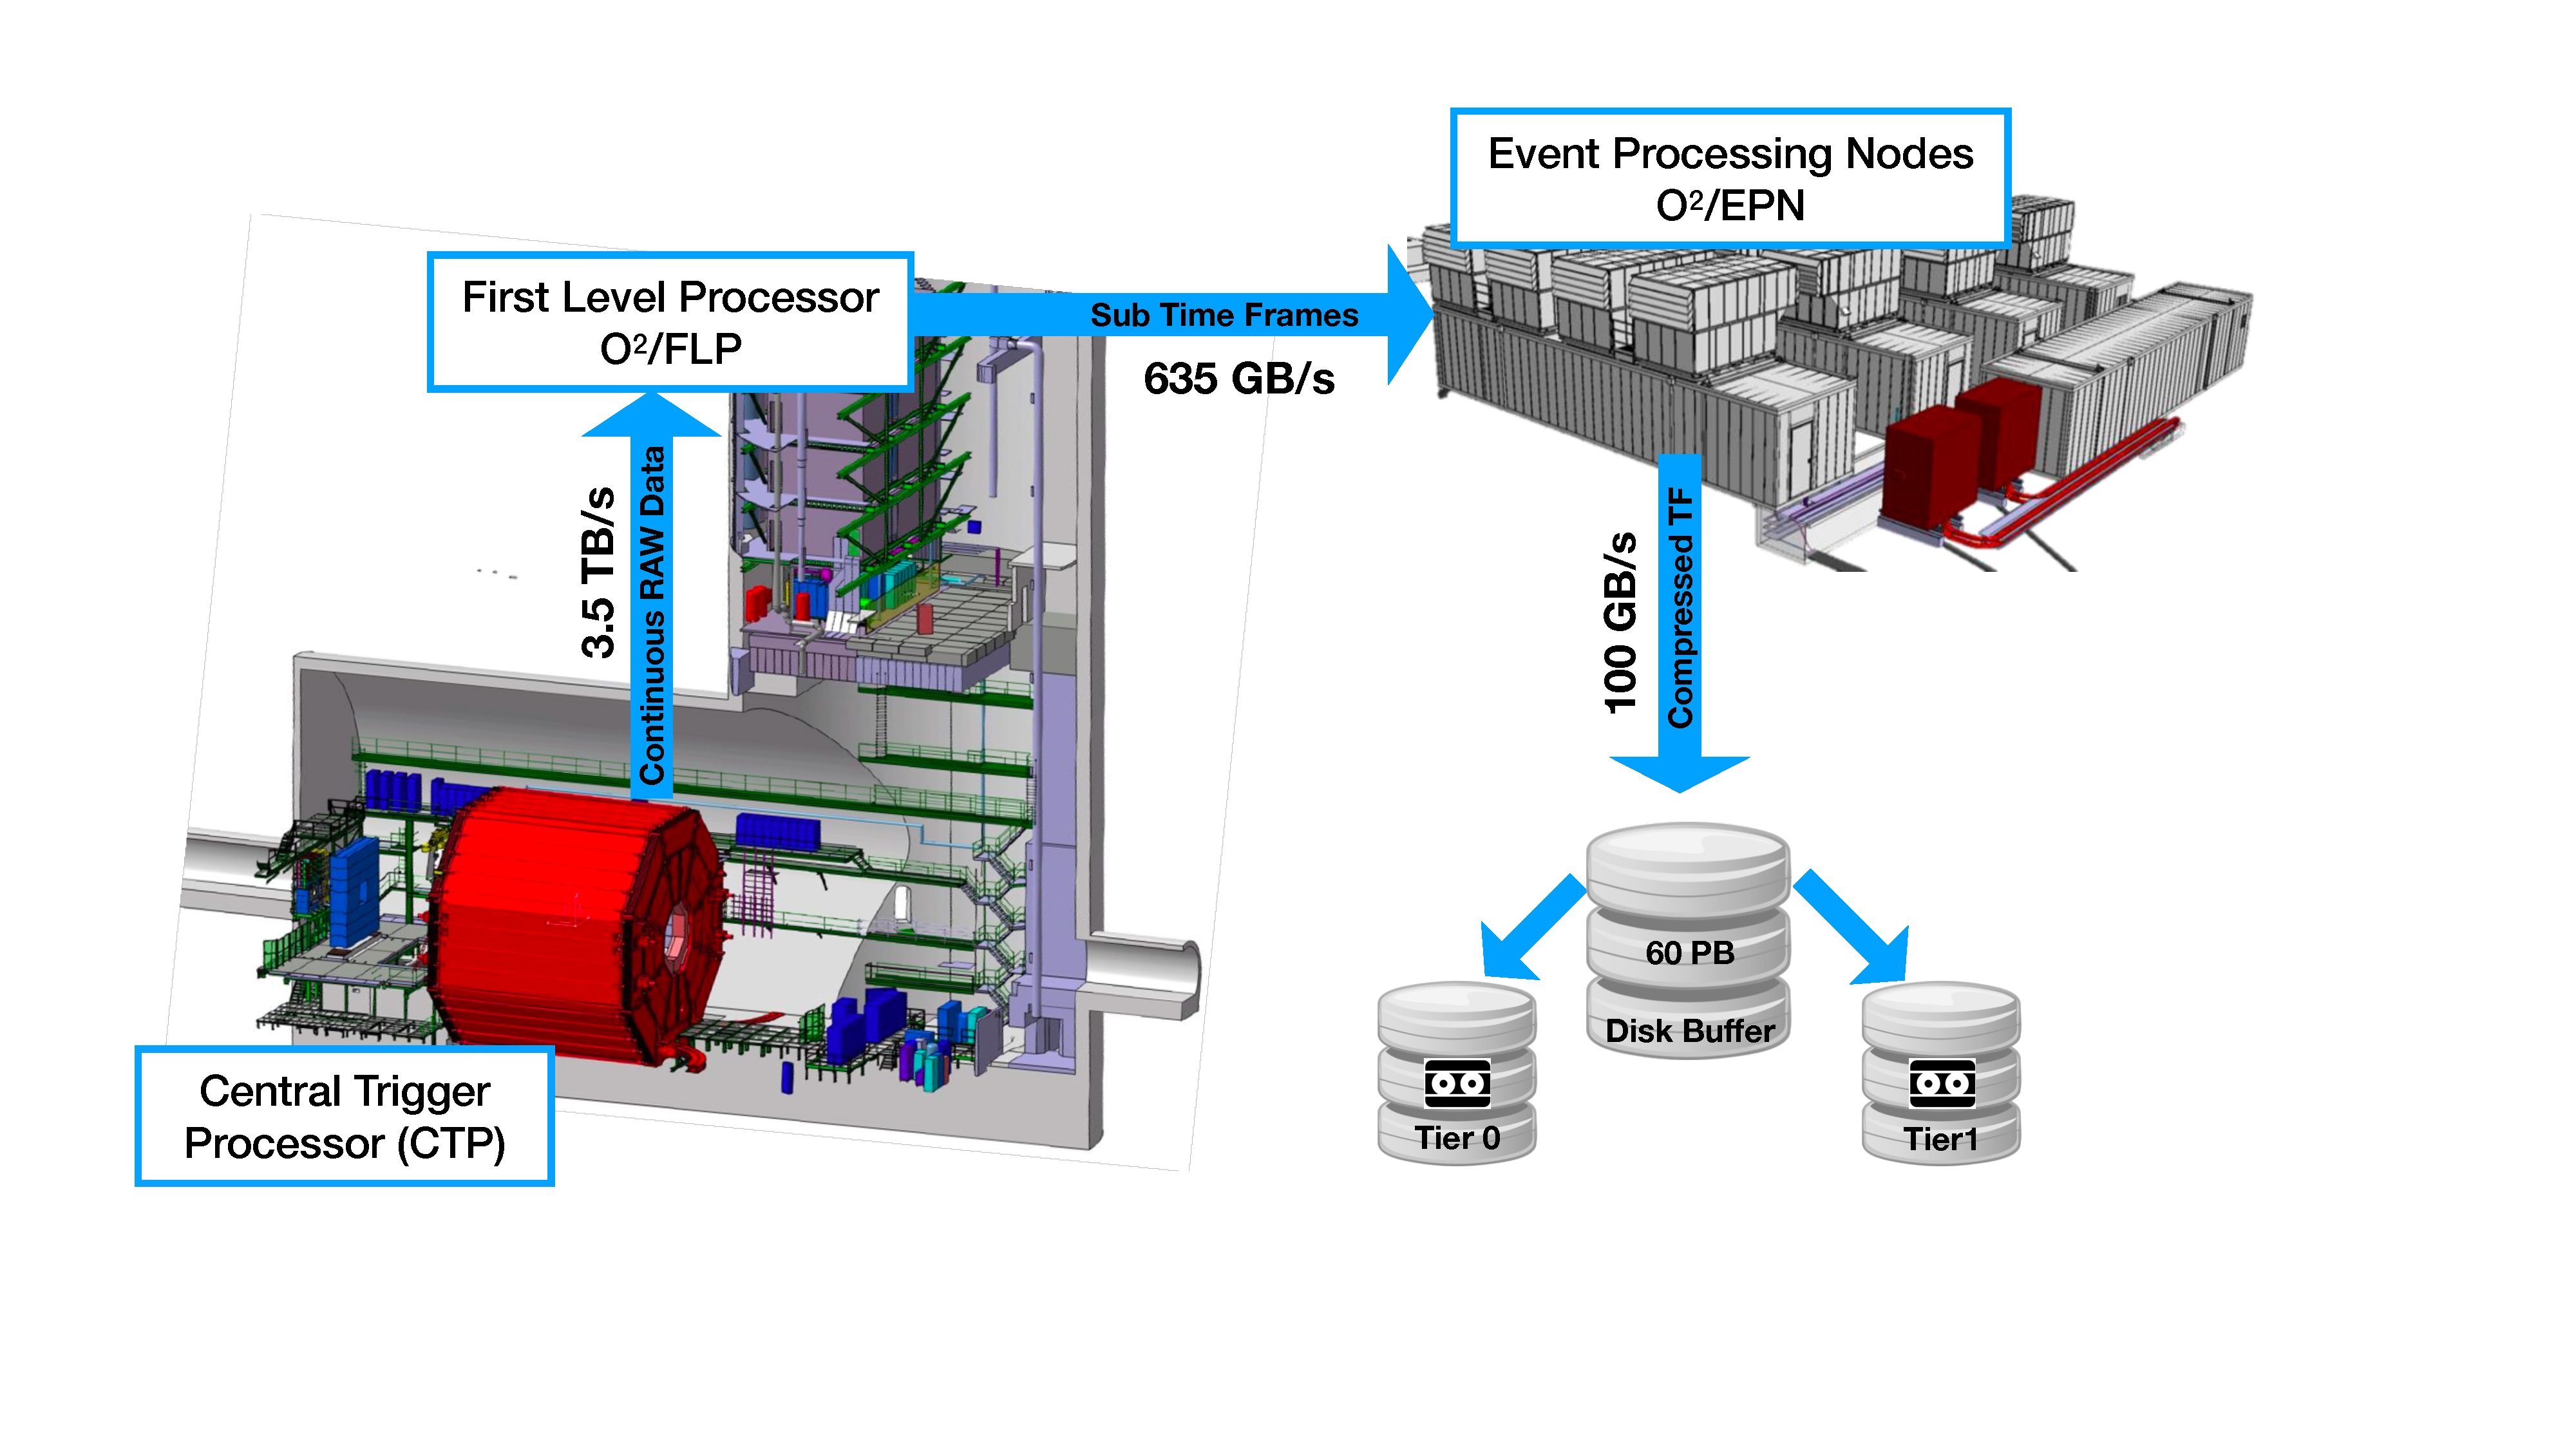
\includegraphics[width=1.\textwidth]{fig/readout/dataFlow.pdf}
  \end{center}
  \caption{O2 Data Processing Overview}
  \label{fig:o2dp}
\end{figure*}

STFs related to the same time period and from all FLPs are received by the same EPN and aggregated into
a complete time frame (TF).
The EPN farm consists of 250 servers hosting each 8 GPUs and
64 CPU cores. The capacity has been dimensioned such that it can achieve
a first pass online synchronous reconstruction, extraction of calibration
objects for subsequent asynchronous reconstruction passes and data reduction.
Data is aggregated into so called compressed time frames (CTF) replacing the original raw data and
written to a
60~PB disk buffer at an output rate of 100~GB/s.
Calibration data from EPNs is aggregated on a dedicated node, processed, and stored in the CCDB. As
for FLP processing, CCDB objects will be distributed back to the whole ${\rm O}^2$ farm through
multi-casting, for usage by the ongoing synchronous reconstruction steps, but also for the later
asynchronous processing and simulation.

Two third of the CTFs are transferred to T0 and one third to T1 for archiving.
After data taking and full detector calibration, at least two asynchronous
reconstruction passes on T0 and T1 centers as well as on the EPN farm are
performed in similar share of 33 \%. The output of these reconstruction passes is stored as Analysis  Object Data (AOD), the input for physics analysis. For specific physics signals, a further data size
reduction and speed-up of the corresponding analyses is achieved by filtering out events of interest and writing out only the minimum event information needed.
The processing of pp data will follow the same chain with the addition of the selection of interesting
events during an asynchronous reconstruction pass with reduction of the CTFs by keeping only the
clusters associated to these events. Reconstruction passes are followed by Monte Carlo production cycles taking into account the time dependent detector conditions.

Besides the compute infrastructure a common software framework has
been developed in collaboration with GSI (FAIR) within which all
online and offline components are developed and operate. It
consists of three main layers.
The {\it Transport Layer} is implemented using the FairMQ message
passing toolkit with FairMQDevices as its main building blocks.
It enables efficient parallelism by providing
abstraction of network and inter process communication as well as
by supporting shared memory backed message passing for devices on the same node. The {\it ${\rm O}^2$ Data
  Model} provides language agnostic and extensible descriptions of messages passed
between devices.
It  provides support for various
back-ends such as a performance optimized simplifies 0-copy format, ROOT based serialisation and Apache Arrow for analysis and and
integration with external tools.
Finally, the {\it Data Processing Layer} (DPL) abstracts computation as a set of data processors
organized in a logical data flow explaining how data is transformed.
Depending on the deployment environment the data
flow is mapped to a concrete topology and from there to a set of processes
running FairMQ devices making sure the configuration matches the deployment
environment.
\begin{figure*}[hbtp]
  \begin{center}
    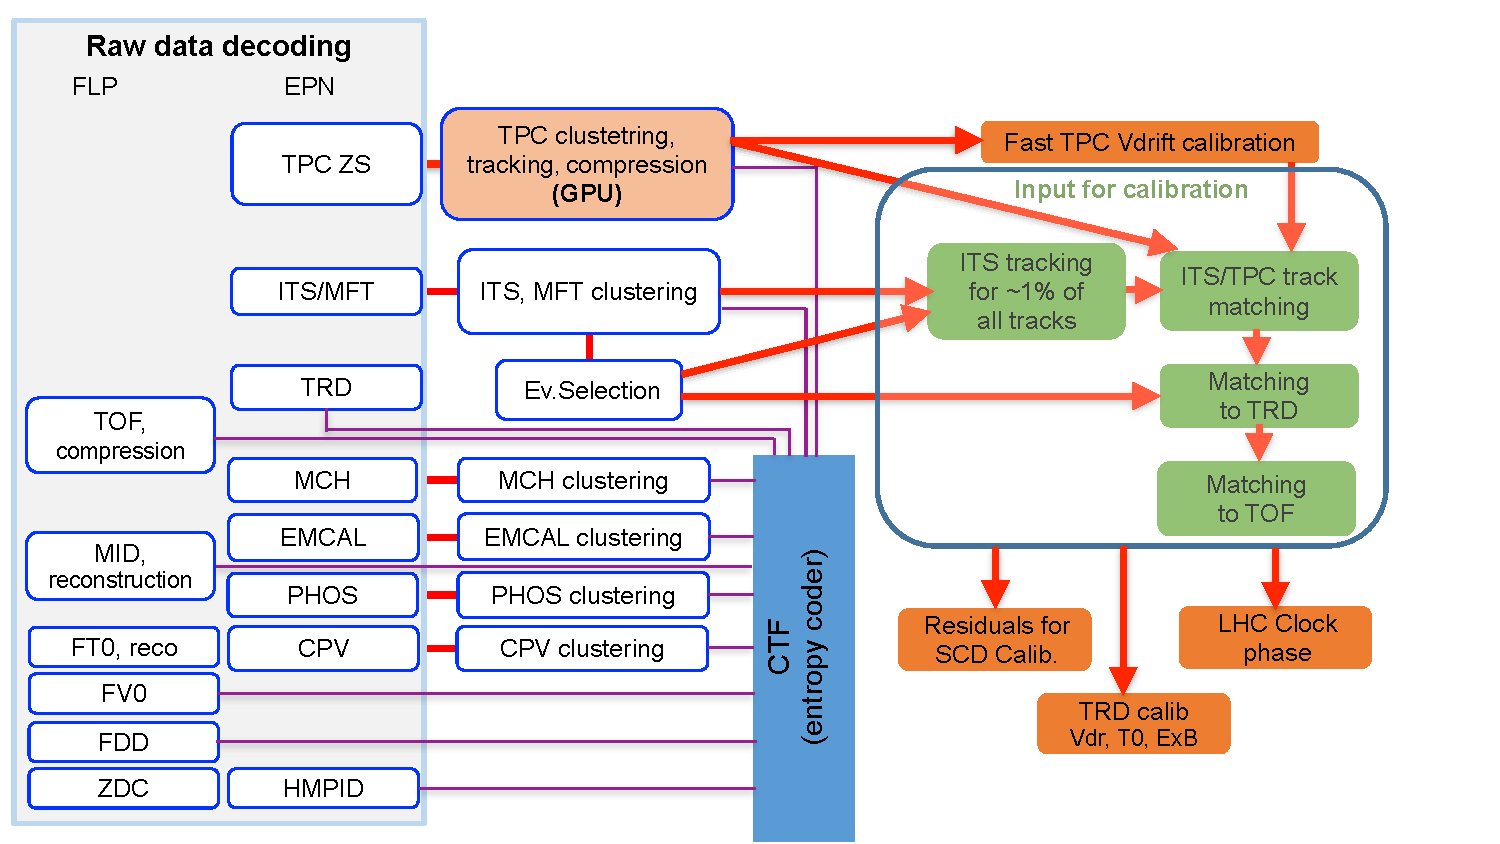
\includegraphics[width=.99\textwidth]{fig/readout/flowSync.pdf}
  \end{center}
  \caption{Synchronous Reconstruction Workflow}
  \label{fig:rwf}
\end{figure*}
\subsubsection{Synchronous Reconstruction}
A schematic representation of the synchronous reconstruction workflow is shown in Fig. \ref{fig:rwf}.
The main objective of synchronous processing is to reduce the data rate from the TPC which is with {\color{blue} 90\%}
the dominant contributor. This is achieved by performing clustering and full track reconstruction in the
TPC and removing background hits from the data. Moreover, cluster space point
coordinates are stored as relative coordinates, thus reducing the entropy and allowing for optimal efficient entropy
encoding of the data.
In addition, detector calibration information is extracted. TPC space charge
distortion calibration uses the information of fully reconstructed barrel tracks including ITS, TOF and
TRD information. However, only a small fraction of all tracks are needed to be fully reconstructed to gain
sufficient statistics. Hence, full TPC reconstruction needed for data compression
is the most compute demanding step. To be able to
reconstruct Pb-Pb collision at a rate of 50~kHz in a cost
effective way it is performed on Graphic Processing Units (GPU). They provide a significant speed-up
with respect to CPU processing (at least a factor of 50 compared to one CPU core) without compromising the physics performance.

\subsubsection{GPU Processing and Data Rejection}
The TPC reconstruction code has been developed starting from the existing Run~2 High Level Trigger (HLT) algorithms.
It starts with the cluster finding and is followed by tracking comprising the track
finding, track merging, fitting and compression steps.
The presence of space charge distortions (SCD) of up to 20~cm
represents a particular challenge for the reconstruction of
continuous data. In absence of triggers which provide a reference for the drift time estimate, the $z$-position of clusters
is unknown. However, this information is needed for the corrections of the SCDs, but also for the determination of the magnetic field strength and the cluster error parameterisation.
Therefore, TPC tracking is first performed without these corrections. Since the distortion effects are
smooth, the track finding is not strongly affected. Track seeds are extrapolated to the beam line
and the most probable $z$-coordinate is calculated under the assumption that the track is from a primary particle and the vertex
is at the interaction point.  The track is refit with the corresponding corrections. The SCD corrections require a first order correction map obtained from simulation or a previous reference run.
Additionally, space charge fluctuations will need to be accounted for, and this will be done by scaling the maps with a granularity of about 5~ms using the charge collected in the TPC (1-dim digital currents) in the previous 160~ms. With these maps cluster positions can be corrected with a precision of \cal{O}(mm) which is sufficient for correct cluster associations to tracks.

Two options for TPC data rejection are supported by the software. In the first
option (A) clusters from identified background (for example from noisy pads or charge clouds
related to low momentum protons) and clusters associated to background tracks, such as very low momentum tracks, loopers and
track segments with large inclination with respect to the TPC padrows, are rejected.  For the second option (B) only clusters attached or
in the proximity of identified signal tracks are kept.
The estimated rejection fractions for options A and B are $12.5-39.1\%$ and $37-53\%$, respectively.
While option B yields lower data size it is more risky in case of calibration problems. Optimal
performance of option A requires identification of hits from particles with momentum below
15~MeV/$c$, which is still under development.

Further data size reduction is achieved by converting the cluster properties from the  single-precision floating point format used in reconstruction to custom integer and floating point formats with exactly as many bits as  needed  for the intrinsic TPC resolution. For entropy reduction, coordinates of hits that are not assigned to tracks
are sorted by geometrical coordinates and the difference to the previous
hit is stored. Raw coordinates (row, pad, time) of hits assigned to tracks
are stored relative to the extrapolated track (Track Model Compression).
Cluster properties, maximum charge, total charge and cluster size, are encoded together in order to profit from their correlation.

While for synchronous reconstruction TPC tracking is by far the most beneficial to be offloaded to GPUs, for the
asynchronous reconstruction passes global reconstruction including ITS tracking will dominate. To this
end other reconstruction components have been already ported to GPU with the final goal to run there
all barrel tracking. The reconstruction code is written using generic C++ code and can run on different
GPU hardware. This opens the possibility to run reconstruction efficiently on heterogeneous
computing platforms that will become available on the GRID:

\subsubsection{\bf CPU Processing}
Synchronous data processing on CPUs is performed in parallel on about 30 cores.
For the ITS and the muon spectrometer system (MFT, MCH, MID) processing starts with space point reconstruction
(clustering). For the barrel calorimeters EMCAL and PHOS, the cell
properties (time, amplitude) are determined by
fitting the raw time distributions. Clusterization is performed in
order to select cells to write to the CTF, while final clustering
will be performed during analysis. Data for time calibration and
dead-channel maps are extracted. For FT0, the reconstruction of
collision time and the vertex $z$-position is performed.

For about 1\% of total tracks selected from peripheral collisions
full tracking including all
barrel detectors is performed, i.e. ITS tracking after clustering,
matching of ITS tracks to TPC tracks
and finally track matching to TRD and TOF. As in Run2, residuals
between
global tracks and TPC clusters are used to create space charge
distortion maps. The sample size is sufficient to provide
Run~2 type correction maps with a granularity of  1-2~min in Pb--Pb and 10~min
in pp.


Global barrel tracks provide also a fast TPC drift
time calibration and TRD calibration (gain, $t_0$, $E \times B$ and drift
velocity). Moreover, the drift of the LHC clock with time (due to temperature
changes that impact the fiber refractive index and the distribution of the LHC clock time to the experiments), which affects the
reference for the Time Of Flight measurement as a global offset,
will be calibrated using global tracks matched to TOF. At the same
time, the TOF channel-level offset in the measured times related to
the cable lengths and electronics will be determined.
During  synchronous processing, input data will be accumulated
for those calibration constants that need significant statistics, are not
important for the the synchronous reconstruction, but are too CPU time demanding to be determined synchronously, like for example, the TOF channel time
slewing. These data will be evaluated before the asynchronous
reconstruction takes place, and the CCDB will be updated.


The final processing step consists in compressing all data stored in the CTF using the rANS algorithm, a variant of
Asymmetric Numeral System coders, which allows to reach the entropy limit.
\subsection{CTP (David; 3p.)}
\subsection{CRU (Tivadar, Alex; 3 p.)}
\subsection{FLP (Pierre; 3p.)}
%
%>>>>>>>>>>>>>>>>>>>>>>>>>>>>>>>>>>>>>>>>>>>>>>>>>>>>>>>>>> The O2/FLP subsystem 
%

The major upgrade of the ALICE experimental apparatus, the resulting dramatic increase of the performance requirements, and the advancement of computing technology have been the major reasons for the design and the implementation of a new computing system called $O^2$ divided in three parts: FLP, EPN and PDP. 

The $O^2$/FLP subsystem includes the First-Level Processors (FLPs) detector read-out farm, the data quality control system and the services for control, configuration, monitoring, logging, and bookkeeping. 
%
%>>>>>>>>>>>>>>>>>>>>>>>>>>>>>>>>>>>>>>>>>>>>>>>>>>>>>>>>>> The FLP farm 
%
\subsubsection{The FLP detector read-out farm}
The read-out farm includes 198 nodes and 490 readout cards (distributed as shown in Table~\ref{tab:flp_farm_links}) for transferring the data from all detectors to the $O^2$ system.

\begin{table}[h!]
\centering
\caption{FLP read-out farm used to transfer the data from the detectors to the $O^2$ system.}
\label{tab:flp_farm_links}
\begin{tabular} { l l r r l r r r}
\hline
Detector &  Link 	&  \multicolumn{2}{c}{Read-out links}  &  \multicolumn{2}{c}{Read-out boards} & Read-out \tabularnewline
         &  type 	& DDL   	& GBT       & C-RORC& CRU	& nodes FLPs \tabularnewline
\hline
CPV     & DDL           &               & ?         &       & 1         &   1 \tabularnewline
CTP     & GBT           &               & 14        &       & 1         &   1 \tabularnewline
DCS     &               &               &           &       &           &   1 \tabularnewline
EMC     & DDL           & 40            &           & 8     &           &   2 \tabularnewline
FIT     & GBT           &               & 34        &       & 3         &   1 \tabularnewline
HMP     & DDL           & 14            &           & 4     &           &   2 \tabularnewline
ITS     & GBT           &               & 495       &       & 24        &  12 \tabularnewline
MCH     & GBT           &               & 550       &       & 30        &  11 \tabularnewline
MFT     & GBT           &               & 304       &       & 11        &   5 \tabularnewline
MID     & GBT           &               & 32        &       & 2         &   1 \tabularnewline
PHS     & DDL           & 16            &           & 4     &           &   2 \tabularnewline
TOF     & GBT           &               & 72        &       & 4         &   2 \tabularnewline
TPC     & GBT           &               & 5832      &       & 361       & 145 \tabularnewline
TRD     & Custom        &               & 1044      &       & 36        &  12 \tabularnewline
ZDC     & GBT           &               & 1         &       & 1         &   1 \tabularnewline
Total   &               & 76            & 8928      & 16    & 474       & 198 \tabularnewline
\end{tabular}
\end{table}
The total nominal read-out performance amounts to 3.4~TB/s from the detector electronics to the read-out boards and the FLP servers. Most of the detectors use the new GBT~\cite{ref_GBT} link and the Common Read-out Unit (CRU)~\cite{ref_CRU_HW, ref_CRU_FW} adopted for this upgrade. The system is also backward compatible with the Detector Data Link (DDL)~\cite{ref_DDL} and the Common Read-Out Receiver Card (C-RORC)~\cite{ref_RORC} used during the LHC Run 1 and 2. 

The server selected for the FLPs is the Dell Poweredge R740. The selection has been done after numerous hardware and software tests~\cite{ref_FLP} and a competitive tender. Each FLP is equipped with 96~GB of DDR memory and 2~CPUs. The CPUs are of two different flavours of the Intel Cascade Lake generation (the Silver 4210 or the Gold 6230 with 10 or 20 hardware cores respectively) depending on the processing needs of the detector. Each FLP hosts up to three CRUs, up to four CRORCs and one Infiniband network interface, each using one PCIe Gen3 x16 slot. The readout software performance allows data to be transferred from 3~CRUs simultaneously at the maximum PCIe Gen3 performance for a total of 330~Gb/s.

The first layer over the PCIe interface to the cards is the PDA (Portable Driver Architecture) UIO (Userspace IO) kernel module~\cite{ref_PDA}. PDA also provides a userspace library in C~\cite{ref_PDA_lib} which supports PCIe device enumeration and provides a handle to PCI devices.
The read-out software includes the readout program and the readoutCard library~\cite{ref_readout} which orchestrate the simultaneous data transfers from the GBT links to the FLP memory and from the memory to the network interface as shown in Fig.\ref{fig_RO}. 
%
\begin{figure}[!h]
\centering
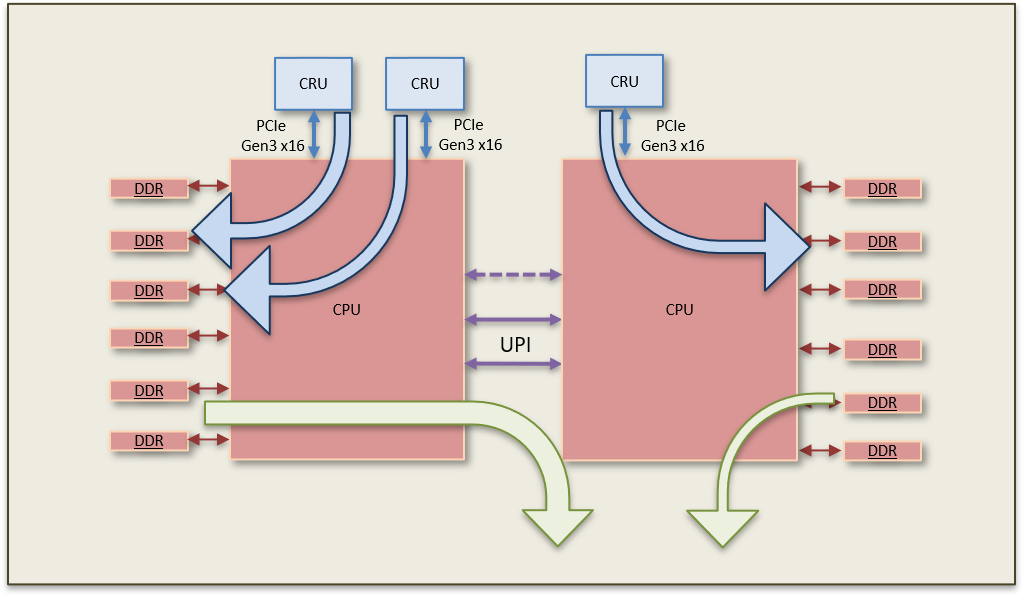
\includegraphics [width=100mm] {o2_flp/Readout_dataflows.png}
\caption{Simultaneous dataflows inside the FLP from the CRUs to the DDR memories and from the memory to the Infiniband network to the EPN farm.}
\label{fig_RO}
\end{figure}
%
 
%
%>>>>>>>>>>>>>>>>>>>>>>>>>>>>>>>>>>>>>>>>>>>>>>>>>>>>>>>>>> The data quality control 
%
\subsubsection{The data quality control}
The online execution of the calibration and the reconstruction and the replacement of the raw input data by reconstructed data, make the need for a reliable data Quality Control (QC) even more essential than usual. Its main motivations are to identify and help overcome problems during data taking and check that the data processing behaves as expected, thus ensuring good quality data for physics analyses.

The $O^2$  QC system \cite{ref_QC} is a distributed software as shown in Fig.\ref{fig_QC}.
    Data samples are selected following a pseudo-random sampling and configurable policies at key points in the data-flow and are dispatched to local (on the FLPs and the EPNs) or remote (on QC servers) QC tasks executing detector-specific algorithms. Their results are published as QC Objects, typically ROOT~\cite{ref_ROOT} histograms. The results of the QC tasks running in parallel on many nodes are assembled by the mergers.  
    Traditional or machine-learning-based checkers evaluate the quality of the objects and produce QC qualities. Finally the QC Objects and the Qualities are stored in the QC repository. This database uses the same technology as the Calibration and Condition DataBase of ALICE $O^2$. The Post-processing component encompasses asynchronous tasks such as correlation and trending of data derived from QC Objects and Qualities and triggered periodically, manually or on certain events (e.g. start of run or end of fill).
    QC and Quality Objects are accessible to shifters and experts through a web-based QC GUI.
%\end{itemize}
%
\begin{figure}[!h]
\centering
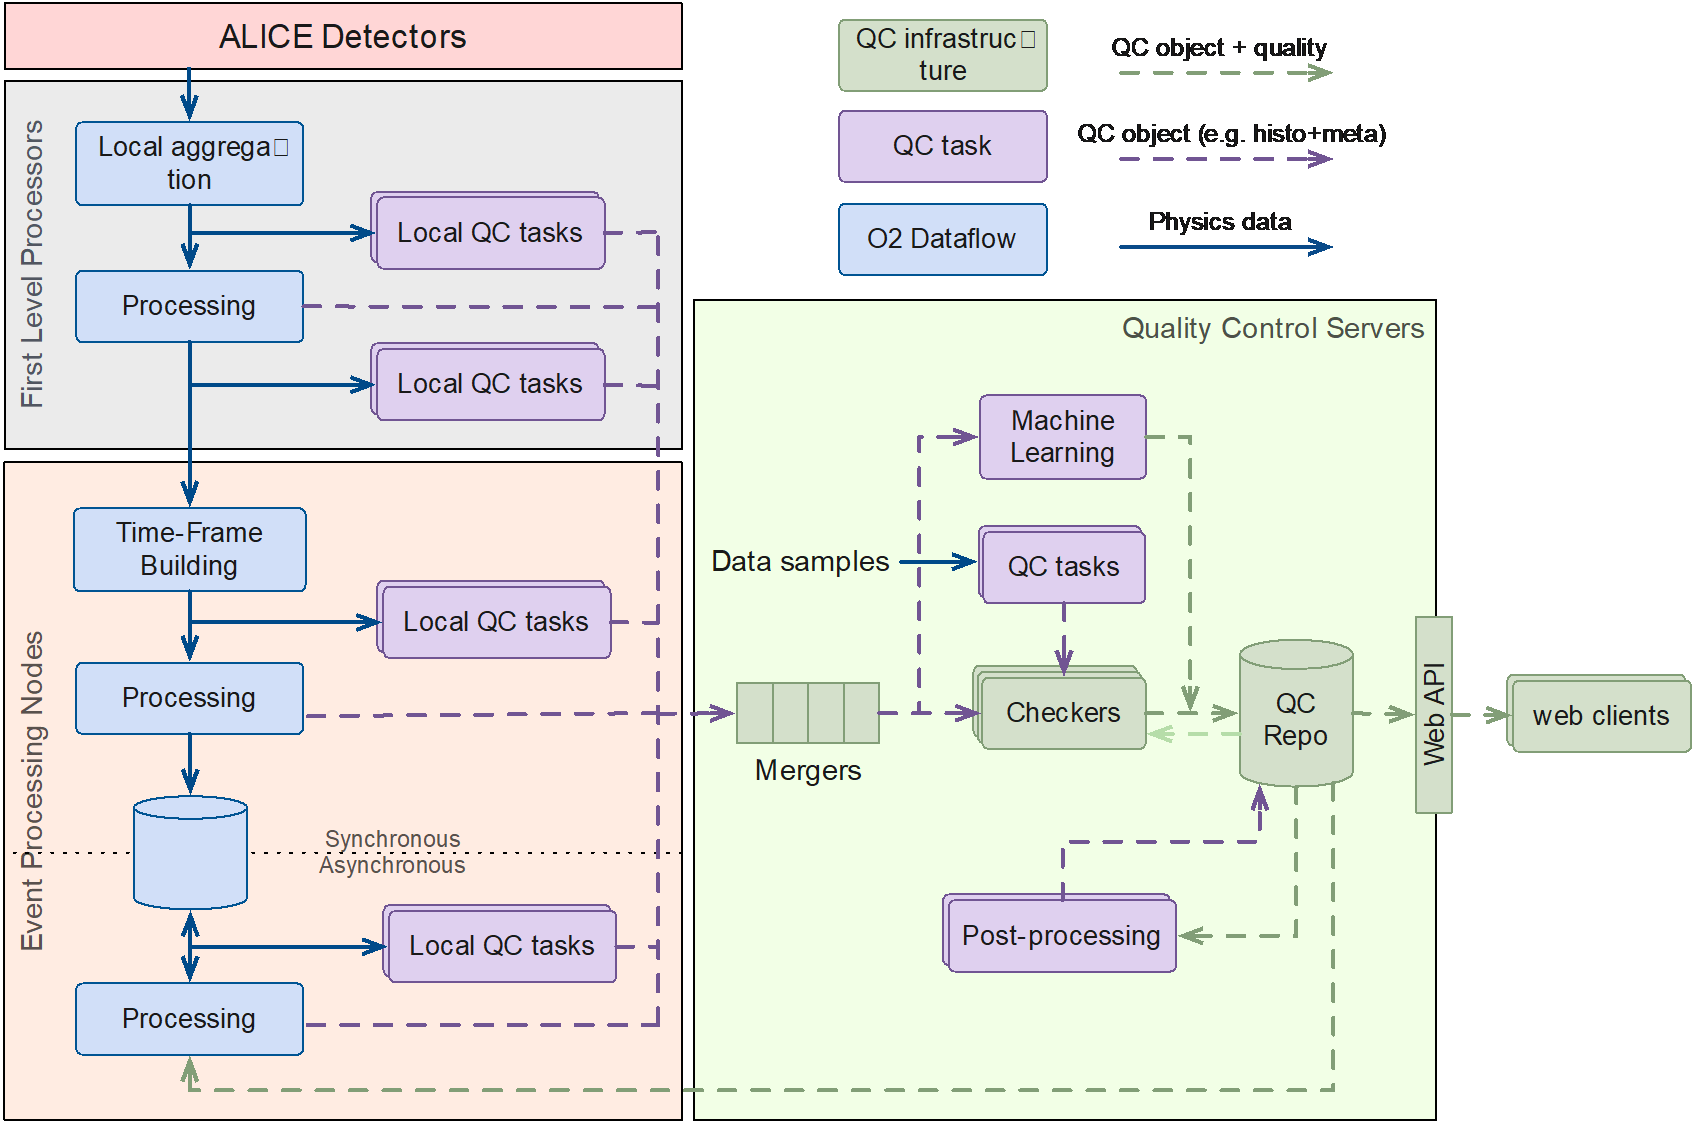
\includegraphics [width=100mm] {o2_flp/QC_Design.png}
\caption{$O^2$ Quality Control design.}
\label{fig_QC}
\end{figure}
%
%>>>>>>>>>>>>>>>>>>>>>>>>>>>>>>>>>>>>>>>>>>>>>>>>>>>>>>>>>> The services 
%
\subsubsection{The services}
%
%>>>>>>>>>>>>>>>>>>>>>>>>>>>>>>>>>>>>>>>>>>>>>>>>>>>>>>>>>> WebUI
\paragraph {Web User Interface framework}
Overview
The Web User Interface (Web UI) framework provides the core functionalities and building blocks to easily create rich web applications.
The server side features REST and WebSocket API, the authentication via CERN single sign-on and the authorisation using CERN e-groups.
The client-side features user interface Cascading Style Sheet building blocks, asynchronous data fetching (Ajax) and bi-directional socket (WebSockets).

%>>>>>>>>>>>>>>>>>>>>>>>>>>>>>>>>>>>>>>>>>>>>>>>>>>>>>>>>>> Control and configuration 
%
\paragraph{Control and configuration}
The ALICE Experiment Control System (AliECS) \cite{ref_aliecs} integrates the experiment control and configuration, the FLP farm control and a high-level control interface to the $O^2$/EPN cluster as shown in Fig~\ref{fig_aliecs}. It implements a distributed state machine to represent the aggregated state of the constituent $O^2$ processes of a data-driven workflow. Furthermore, it allows reconfiguration of running processes and simultaneous operation of multiple worflows, with easy reallocation of resources among workflows. Finally, it reacts promptly to inputs, handling events from the user, the LHC, the trigger system, the DCS, and the cluster itself with a high degree of autonomy. 

AliECS uses FairMQ, part of ALFA \cite{ref_alfa}, which is the common $O^2$ transport layer for physics data.   
Apache Mesos~\cite{ref_mesos} is a cluster resource management system, which facilitates the management of O2/FLP components, resources and tasks inside the O2/FLP facility, 
effectively enabling the developer to program against the datacenter (i.e., the O2/FLP facility at LHC Point 2) as if it was a single pool of resources. 

AliECS interfaces with Consul~\cite{ref_consul}, a key-value store which acts as the system’s configuration repository. The design also includes interfacing with information sources from the LHC, 
the trigger system, and the DCS. Once acquired by the AliECS core, configuration information is processed into an in-memory hierarchical key-value store, and from there it is
fed into a template system in order to generate task deployment and configuration structures.

Most components of AliECS are written in Go~\cite{ref_go}, a statically typed general purpose programming language in the tradition of C, which is particularly suitable for distributed system development because of its advanced synchronization and threading facilities.

\begin{figure}[!h]
\centering
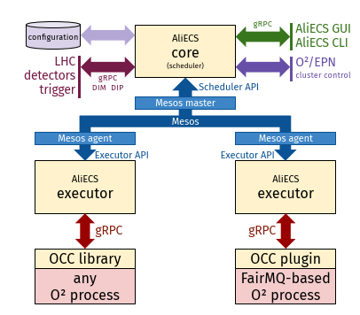
\includegraphics [width=100mm] {o2_flp/AliECS_Design.png}
\caption{AliECS design.}
\label{fig_aliecs}
\end{figure}

%
%>>>>>>>>>>>>>>>>>>>>>>>>>>>>>>>>>>>>>>>>>>>>>>>>>>>>>>>>>> Monitoring 
%
\paragraph{Monitoring}
The monitoring subsystem \cite{ref_monitor1, ref_monitor2} provides a complete overview of the overall system health, detects performance degradation and component failures by collecting, processing, storing and visualising values from hardware and software sensors and probes. As presented in Fig.~\ref{fig_monitoring}, metrics are sent to the system from both Telegraf \cite{ref_telegraf} (for system metrics) and the C++ monitoring library (via Telegraf, for application metrics). These metrics are processed in an Apache Kafka \cite{ref_Kafka} cluster and later written to InfluxDB \cite{ref_influxdb} time-series database for permanent storage.

InfluxDB time-series database supports downsampling which decreases the value resolution over time bringing down the total database size. It is planned to keep high resolution metrics for several days. After that time metrics will be downsampled in order to decrease the number of points and store them until the end of the calendar year. 

The system includes a data visualisation interface based on Grafana \cite{ref_grafana} and channels to email or mattermost for alarms and reporting.
\begin{figure}[!h]
\centering
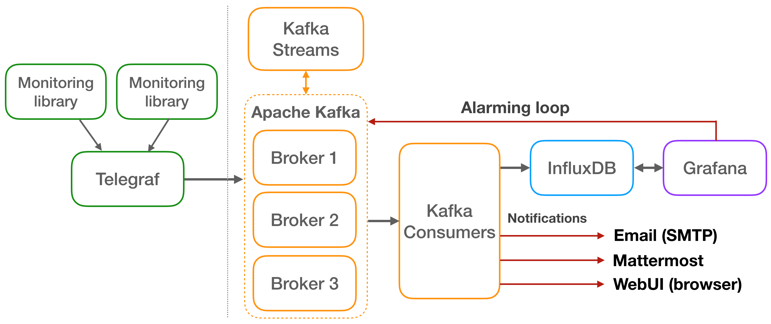
\includegraphics [width=100mm] {o2_flp/Monitoring_Design.png}
\caption{The $O^2$ computing system monitoring design.}
\label{fig_monitoring}
\end{figure}

%
%>>>>>>>>>>>>>>>>>>>>>>>>>>>>>>>>>>>>>>>>>>>>>>>>>>>>>>>>>> Logging 
%
\paragraph{Logging}
The logging system has been adapted from the ALICE Run 2 DAQ software \cite{ref_logging}. A new web-based user interface has been developed in addition to the existing GUIs.
%
%>>>>>>>>>>>>>>>>>>>>>>>>>>>>>>>>>>>>>>>>>>>>>>>>>>>>>>>>>> Bookkeeping 
%
\paragraph{Bookkeeping}
A new bookkeeping system called Jiskefet \cite{ref_bookkeeping} has been developed. It unifies two functionalities: gathering, storing and presenting metadata associated with the operations of the ALICE experiment and tracking the asynchronous processing of the physics data. The front end is based on the WebUI framework like the other applications and is adaptive to various clients such as tablets, mobile devices and other screens. The back end includes an OpenAPI specification based REST API and a relational database.


\subsection{EPN (Volker; 3p.)}
\newpage
\subsection{Grid computing}

\subsubsection{Asynchronous Reconstruction}
Pb--Pb and pp data taking with synchronous reconstruction is followed by an about 4-6 weeks period during which the final calibration constants are evaluated. For some detectors this requires also a short calibration pass over CTF data before the full asynchronous production passes can start.

During reconstruction passes the final calibration is performed, in particular, targeting full correction of TPC distortions and nominal resolution. At this stage, all detectors are included in the reconstruction. The TPC tracks are matched to ITS
tracks and propagated to the outer detectors. The global tracks are established
by combining information from
multiple detectors, and improved track fits are performed.
Primary vertices are reconstructed and secondary vertices are identified in order to
reconstruct V0s and cascade candidates. For long-lived particles decaying at large
radius and producing  TPC tracks unconstrained by other detectors, continuous readout poses an additional challenge. Every pair of unconstrained TPC tracks will need to be
tested for multiple hypotheses of V0s from different primary vertices compatible with
the allowed time (or $z$) range of the tracks. Since the TPC track corrections depend on their $z$ position, this may even require on-the-fly re-calibration and refit of
TPC tracks.  In a final step, the PID hypothesis is assigned combining tracking information from all detectors. For the muon spectrometer system, stand-alone tracking is performed for MFT and
MCH followed by matching of MFT-MCH track-segments and track selection to form global muon tracks. Two full passes of asynchronous reconstruction to achieve the required performance are needed.

The first reconstruction pass over pp data includes an event selection procedure in order to reduce the
overall data size. In addition to physics events of interest, as for example heavy-flavor,
high-multiplicity or diffractive production, events needed for the TPC distortion calibration are
selected. The CTF size is reduced by only keeping the clusters associated to tracks that point to the
primary vertex of a selected collisions withing $\pm 30 \; {\rm cm}$ in $z$. The goal is an event rejection factor of 1000 leading to a CTF reduction of 1.2\% of the original size.

Reconstruction passes are followed by Monte Carlo productions.
Physics Analysis will be performed on the GRID and dedicated analysis facilities. It consumes AODs from data and Monte Carlo productions (including MC truth)
and produces additional physics object like fully reconstructed charmed hadrons and jets.

\subsubsection{Simulation}
Physics simulation comprises primary event simulation, the transport of particles through the detector
geometry, detector response simulation and digtisation of the detector signals.
The ${\rm O}^2$ software framework for simulation has been developed withing the ALFA project, a ALICE/FAIR
collaborative effort based on common components such as FairRoot and FairMQ.

GEANT4 is employed as the main transport engine. As for AliRoot in Run~1/2 the ${\rm O}^2$ simulation
framework uses external transport codes through the Virtual Monte Carlo (VMC) layer. This
allows to use also Geant3 and FLUKA with the same user code, for example for systematic
studies or radiation calculations. The detector geometry is described using ROOT/TGeo and
the detector response using the VMC API and callbacks. As part of new developments for ${\rm O}^2$
the VMC interface has been extended to interfacing fast detector
simulation components which can replace detailed simulation in parts of the detector or
for certain particle types. Preserving the VMC interface has allowed efficient porting of user code from AliRoot into ${\rm O}^2$.

The ${\rm O}^2$ simulation framework has been developed with two main objectives
in mind: the possibility to leverage opportunistic resources, in
particular HPC, which frequently offer only very short processing time
windows and performance optimization through parallelism on top of the capability of individual parts, going beyond standard event multi-threading of Geant4.
To this end the simulation process is broken up into individual actors:
primary particle generation (event server), simulation workers and I/O
processes. Actors are asynchronous processes that can interact with each
other via sending and receiving messages. Parallelism is achieved by
further dividing the event simulation task into the processing of
sub-events. Multiple independent simulation worker devices are
instantiated at the same time. Each of those actors asks the event
server for work chunks to process, where a chunk is either a full event
or a sub-event. Hence, the system is able to process multiple events in
parallel or collaborate on the simulation of a single event
concurrently. A strategy based on so called late forking makes optimal use of common memory between the different processes. Processing speed-up as a function of simulation workers shows almost ideal strong
scaling. By reducing the processing time for a unit of work, the framework naturally supports the usage of opportunistic resources providing short processing time windows.

The output of detector response simulations are hits typically containing space-point
and energy loss information of particles passing sensitive detectors. They serve as the
input to digitization. Since at the peak Pb--Pb luminosity up to about 10 events can
overlap withing the drift-time of the TPC a simulated time frame cannot be assembled
from independently digitized events. Hence, the digitisation workflow takes into
account the contributions from different collisions to the same digits.

Since the full simulation of Pb-Pb collisions is very time consuming an optimized
simulation strategy, named embedding, has been developed for AliRoot and used in
production during Run~2. Pb--Pb background events are simulated and the output is
used several times in order to overlap rare signal events. Owing to the overlapping features
mentioned above the ${\rm O}^2$ simulation framework supports this strategy naturally. The maximum time gain by embedding is limited by the time spent in digitizationn, in particular of the TPC.
For this reason effort has been put into reducing digitization time to a minimum.

\subsubsection{Analysis}
In Run~3 about 10~PB of analysis object data (AOD) will be produced per Pb--Pb running period and
a total of about 50~PB will be accumulated in Run~3 and 4. Considering a typical analysis
turnaround cycle of a few days for the full data set, a data throughput of the order of up to
100~GB/s is required. In order to meet this requirement an optimized analysis model as well as a
new analysis framework have been designed.

In order to achieve a fast turnaround cycle for analysis code validation and cut
optimization, 10\% of each data set including simulated data is copied to a
dedicated Analysis Facility (AF). The Analysis Facility consists of 20000 cores,
equipped with fast local storage and an internal network capable of sustaining
high rates of data transfer from the storage to the the computing nodes. The
facility only analyzes local data, to reduce problems due to slow network
connections or remote storage instabilities. The fast internal network allows for
data to be moved quickly from the storage to the nodes. Only analysis tasks that
have been validated on the AF are allowed to participate in analysis over complete data
sets on the GRID, avoiding inefficiencies in the most costly stage of processing.
Moreover, a large reduction of processing time is expected from the systematic
usage of so called derived data sets of reduced size. This is in particular the
case for analysis of rare processes.
Derived data sets can be obtained through event selection (filtering) and/or event
data reduction (selection of only those quantities strictly needed for a specific analysis).

The new data analysis framework fully leverages the  Data Processing
Layer and is built on top of it  offering an even higher level of abstraction for the benefit of analysis code writers.
As in Run~2, analysis is organized in trains consisting of wagons, the individual analysis tasks. In the new framework wagons correspond to a group of DPL devices allowing to process the tasks in parallel and to remove crashing tasks from the train.
Data is represented in memory as flat tables similar to a relational database and is stored as flat
root trees. This saves the processing time for de-serialization needed for the nested C++ objects used in the old framework.
In order to keep the size on disk small, a number of quantities are recomputed automatically when the data is read from disk. Significant development has been done to perform these operations transparent to the user (building on C++17 extensions).
The in-memory tables are implemented using Apache Arrow, an Open Source cross-language
development platform. It provides inter operability between external tools like Python Pandas,
Sparks and many others. The compatibility with ROOT is guaranteed by using the TArrowDS data
source which allows using Arrow with TDataFrame. Besides I/O efficiency the new data format
naturally allows for optimized vectorized processing and declarative analysis.
The frameworks API isolates many of the advanced features from the user and data access methods are similar to the ones used in the Run~1/2 framework. This facilitates porting of user analysis code into the new framework.
\end{document}
~
